\documentclass[letterpaper, reqno,11pt]{article}
\usepackage[margin=1.0in]{geometry}
\usepackage{color,latexsym,amsmath,amssymb,graphicx,float,listings,tikz}
\usepackage{hyperref}

\hypersetup{
colorlinks=true,
linkcolor=magenta,
filecolor=magenta,
urlcolor=cyan,
}

\graphicspath{ {images/} }

\begin{document}
\pagenumbering{arabic}
\title{Math 406 Homework 2}
\date{10/10/23}
\author{Xander Naumenko}
\maketitle

{\medskip\noindent\bf Question 1.} See tables \ref{tab:q1a}, \ref{tab:q1b}, \ref{tab:q1c}, \ref{tab:q1d} and \ref{tab:q1e} for the required tables. For the log-log plots see figures \ref{fig:q1a}, \ref{fig:q1b}, \ref{fig:q1c}, \ref{fig:q1d} and \ref{fig:q1e}.

From in class, we derived that the error for midpoint is $O(h^{2})$, trapezium is $O(h^{2})$, Simpson is $O(h^{4})$ and Gauss-Legendre is $O(h^{2N})=O(h^{6})$. However, for specific integrals the integrand may help particular methods more than others, as those bounds are all worst cases. For part a in figure \ref{fig:q1a} we see the ``expected'' behavior, with midpoint and trapezium behaving almost identically, Simpson falling faster and Gauss-Legendre even faster.

Part b in figure \ref{fig:q1b} is a bit odd, as by pure coincidence all the methods arrive at the precisely correct value for $N=4,16,32$. This is pure numerical fortuity though, this doesn't reflect a general reason these methods should do well in the worst case. Part c and d in figures \ref{fig:q1c} and \ref{fig:q1d} are similar, with the noticeable difference that the midpoint rule behaves almost identically to Simpson in part d. Finally for part e in figure \ref{fig:q1e}, trapezium/Simpson don't work and only Gauss-Legendre beats Midpoint as expected.

The code for this question can be seen here:
\begin{lstlisting}
disp('midpoint')
numerical_integration(-1, 1, @(x) 1/(1+x^2)^0.5, 32, 1);
disp('trap')
numerical_integration(-1, 1, @(x) 1/(1+x^2)^0.5, 32, 2);
disp('simpson')
numerical_integration(-1, 1, @(x) 1/(1+x^2)^0.5, 32, 3);
disp('gauss_legendre')
numerical_integration(-1, 1, @(x) 1/(1+x^2)^0.5, 32, 4);
disp('real')
% -2*log(2^0.5-1)

functions = {@(x) 1/(1+x^2)^0.5, @(x) sin(2*x)^2, @(x) x^(4.0/3), @(x) x^(1.0/3), @(x) (-log(x))^0.5};
bounds = [-1,1; 0,pi; 0,1; 0,2; 0,1];
real_ans = [-2*log(2^0.5-1), pi/2, 3.0/7, 3/(2^(2.0/3)), pi^0.5/2];
Ns = [2,4,16,32];
tables = zeros(5,4,5);
for i = 1:length(functions)
    f = functions{i};
    for j = 1:length(Ns)
        N = Ns(j);
        for choice = [1,2,3,4]
            if i ~= 5 || (choice ~= 2 && choice ~= 3)
                tables(i,j,choice) = numerical_integration(bounds(i,1),bounds(i,2),f,N,choice);
            end
        end
        tables(i,j,5) = real_ans(i);
    end
end

for i = 1:5
    disp(array2table(squeeze(tables(i,:,:))))
end


% Calculate the errors
errors = abs(tables - real_ans');

methods = {'Midpoint', 'Trapezium', 'Simpson', 'Gauss-Legendre'};
colors = {'r', 'g', 'b', 'k'};

for func_idx = 1:5
    figure('Name', ['Function ' num2str(func_idx)]); % Creates a new figure for each function
    hold on;
    for choice = 1:4
        loglog(Ns, squeeze(errors(func_idx, :, choice)), '-o', 'Color', colors{choice}, 'DisplayName', methods{choice});
    end
    xlabel('N');
    ylabel('Error');
    title(['Log-Log plot of N vs Error for Function ', num2str(func_idx)]);
    
    % Ensuring that the axes are in log-log scale
    set(gca, 'XScale', 'log', 'YScale', 'log');
    
    legend('Location', 'southwest');
    grid on;
    hold off;
end

% 1. Midpoint rule with N cells
% 2. Trapezium rule with N cells
% 3. Simpson''s rule with 2N cells
% 4. Three-point Gauss-Legendre quadrature with N cells
function result = numerical_integration(a, b, f, N, choice)

    switch choice
        case 1
            result = midpoint_rule(f, a, b, N);
        case 2
            result = trapezium_rule(f, a, b, N);
        case 3
            result = simpsons_rule(f, a, b, N);
        case 4
            result = gauss_legendre(f, a, b, N);
        otherwise
            return;
    end

    % fprintf('The result of the integration is: %.5f\n', result);
end

function result = midpoint_rule(f, a, b, N)
    result = 0;
    for i = 0:(N-1)
        point = a+(i+0.5)*(b-a)/N;
        result = result + f(point);
    end

    result = result * (b-a)/N;
end


function result = trapezium_rule(f, a, b, N)
    result = 0;
    for i = 1:(N-1)
        point = a+i*(b-a)/N;
        result = result + 2*f(point);
    end
    result = result + f(a) + f(b);

    result = result * (b-a)/N/2;
end

function result = simpsons_rule(f, a, b, N)
    result = 0;
    for i = 1:N
        left = a+(i-1)*(b-a)/N;
        right = a+i*(b-a)/N;
        result = result + 1/3*(b-a)/N/2*(f(left)+4*f((left+right)/2)+f(right));
    end
end

function result = gauss_legendre(f, a, b, N)
    x = [-sqrt(3/5), 0, sqrt(3/5)];
    w = [5/9, 8/9, 5/9];

    result = 0;
    for i = 1:N
        left = a + (i-1)*(b-a) / N;
        right = a + i*(b-a)/N;
        for j = 1:3
            xi = 0.5*(left+right + (right-left) * x(j));
            result = result+w(j)*f(xi);
        end
    end
    result = 0.5 * (b-a)/N*result;
end
\end{lstlisting}

\begin{table}
\centering
\begin{tabular}{|c|c|c|c|c|}
\hline
$N$ & Midpoint & Trapezium & Simpson & Gauss-Legendre \\
\hline
2 & 1.78885438199983 & 1.70710678118655 & 1.76160518172874 & 1.76266240387583 \\
\hline
4 & 1.77014250014533 & 1.74798058159319 & 1.76275519396128 & 1.76274697462844 \\
\hline
16 & 1.76320768598367 & 1.7618262836833 & 1.76274721855022 & 1.76274717401768 \\
\hline
32 & 1.76286227284615 & 1.76251698483349 & 1.76274717684193 & 1.76274717403875 \\
\hline
\end{tabular}
\caption{Question 1a}
\label{tab:q1a}
\end{table}

\begin{table}
\centering
\begin{tabular}{|c|c|c|c|c|}
\hline
$N$ & Midpoint & Trapezium & Simpson & Gauss-Legendre \\
\hline
2 & 3.14159265358979 & 7.06745147303987e-32 & 2.0943951023932 & 1.60606730241802 \\
\hline
4 & 1.5707963267949 & 1.5707963267949 & 1.5707963267949 & 1.5707963267949 \\
\hline
16 & 1.5707963267949 & 1.5707963267949 & 1.5707963267949 & 1.5707963267949 \\
\hline
32 & 1.5707963267949 & 1.5707963267949 & 1.5707963267949 & 1.5707963267949 \\
\hline
\end{tabular}
\caption{Question 1b}
\label{tab:q1b}
\end{table}

\begin{table}
\centering
\begin{tabular}{|c|c|c|c|c|}
\hline
$N$ & Midpoint & Trapezium & Simpson & Gauss-Legendre \\
\hline
2 & 0.419455176774456 & 0.448425131496025 & 0.429111828348312 & 0.428525592513674 \\
\hline
4 & 0.426049167558007 & 0.43394015413524 & 0.428679496417085 & 0.428562331914328 \\
\hline
16 & 0.428391866554757 & 0.428943359698886 & 0.4285756976028 & 0.428571070406974 \\
\hline
32 & 0.428524607238247 & 0.428667613126822 & 0.428572275867772 & 0.428571357502592 \\
\hline
\end{tabular}
\caption{Question 1c}
\label{tab:q1c}
\end{table}

\begin{table}
\centering
\begin{tabular}{|c|c|c|c|c|}
\hline
$N$ & Midpoint & Trapezium & Simpson & Gauss-Legendre \\
\hline
2 & 1.93841476853743 & 1.62996052494744 & 1.83559668734077 & 1.89373800719319 \\
\hline
4 & 1.91040464923353 & 1.78418764674243 & 1.86833231506983 & 1.89141202322811 \\
\hline
16 & 1.89332086475362 & 1.8728210349583 & 1.88648758815518 & 1.89012260552418 \\
\hline
32 & 1.89126652809474 & 1.88307094985596 & 1.88853466868182 & 1.8899772279319 \\
\hline
\end{tabular}
\caption{Question 1d}
\label{tab:q1d}
\end{table}

\begin{table}
\centering
\begin{tabular}{|c|c|c|c|c|}
\hline
$N$ & Midpoint & Trapezium & Simpson & Gauss-Legendre \\
\hline
2 & 0.856885021909063 & 0 & 0 & 0.881394330687781 \\
\hline
4 & 0.870845677383917 & 0 & 0 & 0.883847456341008 \\
\hline
16 & 0.882289474604227 & 0 & 0 & 0.885658742625317 \\
\hline
32 & 0.884274758802113 & 0 & 0 & 0.88595040876536 \\
\hline
\end{tabular}
\caption{Question 1e}
\label{tab:q1e}
\end{table}

\begin{figure}[htpb]
    \centering
    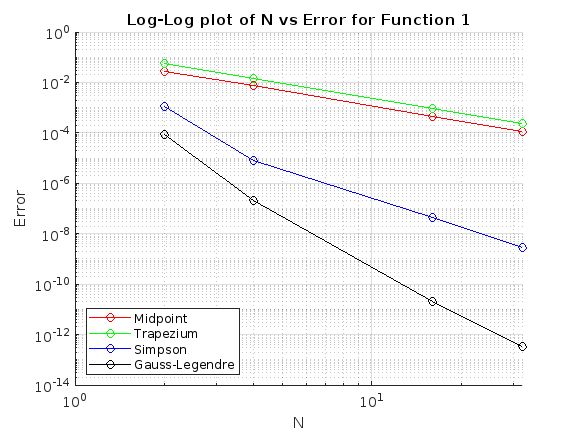
\includegraphics[width=0.8\textwidth]{q1a}
    \caption{Error of Question 1a.}
    \label{fig:q1a}
\end{figure}
\begin{figure}[htpb]
    \centering
    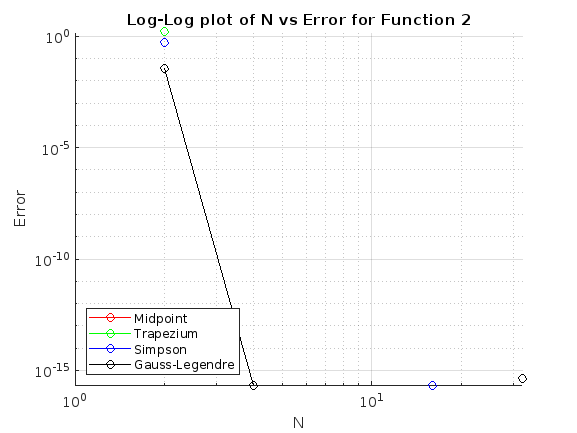
\includegraphics[width=0.8\textwidth]{q1b}
    \caption{Error of Question 1b. Note that due to the fact that the error goes to zero very quickly for the different methods by chance means this plot doesn't look like the others.}
    \label{fig:q1b}
\end{figure}
\begin{figure}[htpb]
    \centering
    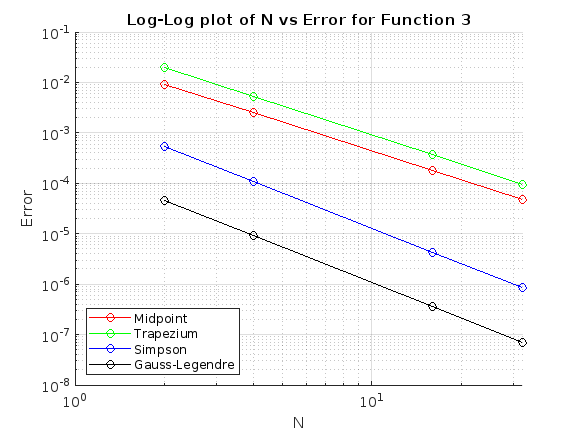
\includegraphics[width=0.8\textwidth]{q1c}
    \caption{Error of Question 1c.}
    \label{fig:q1c}
\end{figure}
\begin{figure}[htpb]
    \centering
    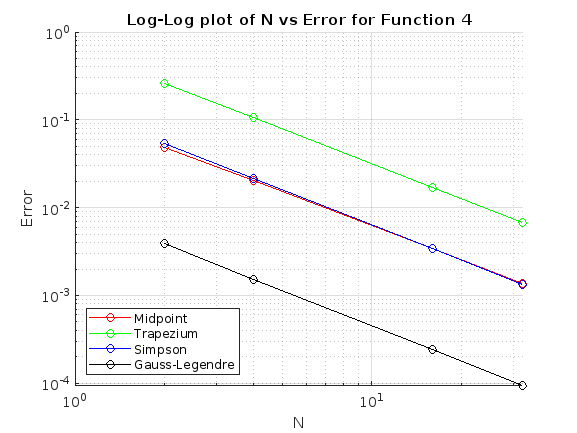
\includegraphics[width=0.8\textwidth]{q1d}
    \caption{Error of Question 1d.}
    \label{fig:q1d}
\end{figure}
\begin{figure}[htpb]
    \centering
    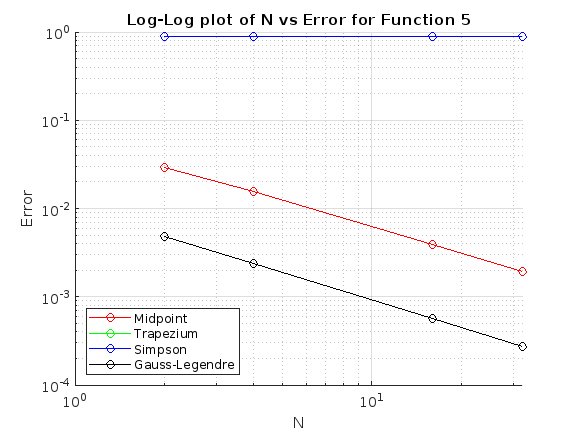
\includegraphics[width=0.8\textwidth]{q1e}
    \caption{Error of Question 1e. Ignore the error for trapezium/Simpson, they were set to 0 in the code so had a constant error.}
    \label{fig:q1e}
\end{figure}

{\medskip\noindent\bf Question 2.} Using the given asymptotic expansion for the Trapezium rule error, we get
\[
I(0)-I(h_{s+1})=I(0)-I(\frac{1}{2}h_s)=\sum_{i=1}^{\infty}\frac{1}{2^{2i}}c_ih_s^{2i}
\]
\[
\implies 4I(\frac{1}{2}h_s)=4I(0)-\sum_{i=1}^{\infty}\frac{1}{2^{2i}}c_ih_s^{2i}
\]
\[
\implies I(0)=\frac{4I(\frac{h_2}{2})-I(h_2)}{3}+ \sum_{i=2}^{\infty}\frac{2^{2(i-1)}-1}{3\cdot 2^{2(i-1)}}c_i h_s^{2i}
.\]
Define $a_s^{(1)}=I(h_s)$ and $c_i^{(2)}$ as in the question. Then simply rearranging the above formula algebraically, we get
\[
I(0)-\left(I(\frac{h_2}{2})+\frac{I(\frac{h_2}{2})-I(h_s)}{3}\right)=I(0)-a_{s+1}^{(1)}-\frac{a_{s+1}^{(1)}-a_s^{(1)}}{3}=I(0)-a_{s}^{2}=\sum_{i=2}^{\infty}c_{i}^{(2)}h_s^{2i}
\]
as required. To eliminate the $O(h^{4})$ term we can again rearrange, this time leaving off some algebra and leaving $c_i^{(3)}$ to be defined in the next part:
\[
I(0)-a_{s+1}^{2}+ \frac{a_{s+1}^{2}-a_s^{m-1}}{15}=\sum_{i=3}^{\infty}c_i^{(3)}h_s^{2i}
.\]

To find the general recursion formula, we follow a similar process to what we just did. We've already shown the result $m=2$, using recursion we just need to prove that the result holds for $m$ given that it holds for $m-1$. Assume that for some $m$,
\[
    I(0)-a_{s}^{(m-1)}=\sum_{i=m-1}^{\infty}c_i^{(m-1)}h_s^{2i}
\]
and
\[
    I(0)-a_{s+1}^{(m-1)}=\sum_{i=m-1}^{\infty}\frac{1}{2^{2i}}c_i^{(m-1)}h_{s}^{2i}
.\]
Subtracting these, we get
\[
I(0)-\frac{(4^{m-1})a_{s+1}^{(m-1)}-a_s^{(m-1)}}{4^{m-1}-1}=\sum_{i=m}^{\infty}\left((\frac{1}{4^{i-1}}-1)\frac{1}{4^{m-1}-1}c_i^{(m-1)}\right)h_s^{2i}
.\]
Define $c_i^{(m)}=\left((\frac{1}{4^{i-1}}-1)\frac{1}{4^{m-1}-1}c_i^{(m-1)}\right)$. Then the previous equation is equivalent to
\[
I(0)-a_{s+1}^{(m-1)}-\frac{a_{s+1}^{(m-1)}-a_s^{(m-1)}}{4^{m-1}-1}=\sum_{i=m}^{\infty}c_{i}^{m}h_s^{2i}
.\]
Thus clearly we have that $a_s^{(m)}=a_{s+1}^{(m-1)}+\frac{a_{s+1}^{(m-1)}-a_s^{(m-1)}}{4^{m-1}-1}$ as required.

For the coding portion, the table for a tolerance of $1\cdot 10^{-5}$ can be seen in table \ref{tab:q2}. Note that my interpretation of tolerance was when successive Richardson extrapolants differed by at most the tolerance. It took 3 refinements (including the first estimate $a_s^{(0)}$, if you don't count that then 2) to arrive at 5 digits of accuracy, but due to the way I calculated tolerance the function returns $a_s^{(3)}$. The plot of the values used can be seen in figure \ref{fig:q2}. The code used was:

\begin{lstlisting}
f = @(x)1./(4+x.^2)
[Integral, I, X] = Romberg(f,0,1,0.00001,4)
disp(I)
disp(X)
disp(0.5*atan(0.5))

scatter(X, f(X))
title('Function Evaluation Points for Romberg Integration')

function [Integral,I,X] = Romberg(f,a,b,tol,kmax)
  I = zeros(kmax, kmax+1);
  for s=1:kmax
    I(s,1) = (b-a)/2^(s-1);
    % I(s,2) = trapez(f,a,b,2^(s-1));
  end

  k = 1;
  I(1,2) = trapez(f,a,b,1);
  I_last = I(2,1)+2*tol;
  I_cur = I(2,1);
  while abs(I_cur - I_last) >= tol && k<kmax
    k = k+1;
    I(k,2) = trapez(f,a,b,2^(k-1));
    for m=1:k-1
      I(k-m,m+2) = I(k-m+1,m+1) + (I(k-m+1,m+1)-I(k-m,m+1))/(4^m-1);
    end
    I_last = I_cur;
    I_cur = I(1,k+1);
  end

  Integral = I_last;
  X = a:(b-a)/2^(k-1):b;
end


function result = trapez(f, a, b, N)
    result = 0;
    for i = 1:(N-1)
        point = a+i*(b-a)/N;
        result = result + 2*f(point);
    end
    result = result + f(a) + f(b);

    result = result * (b-a)/N/2;
end

\end{lstlisting}

\begin{table}[ht]
\centering
\caption{Values for question 2.}
\label{tab:q2}
\begin{tabular}{cccccc}
\hline
$h$ & $a_s^{(0)}$ & $a_s^{(1)}$ & $a_s^{(2)}$ & $a_s^{(3)}$ \\
\hline
1. & 0.225000000000000 & 0.231862745098039 & 0.231823901320275 & 0.231823801752296 \\
0.5 & 0.230147058823529 & 0.231826329056385 & 0.231823803308046 & 0 \\
0.25 & 0.231406511498171 & 0.231823961167317 & 0 & 0 \\
0.125 & 0.231719598750030 & 0 & 0 & 0 \\
\hline
\end{tabular}
\end{table}

\begin{figure}[htpb]
    \centering
    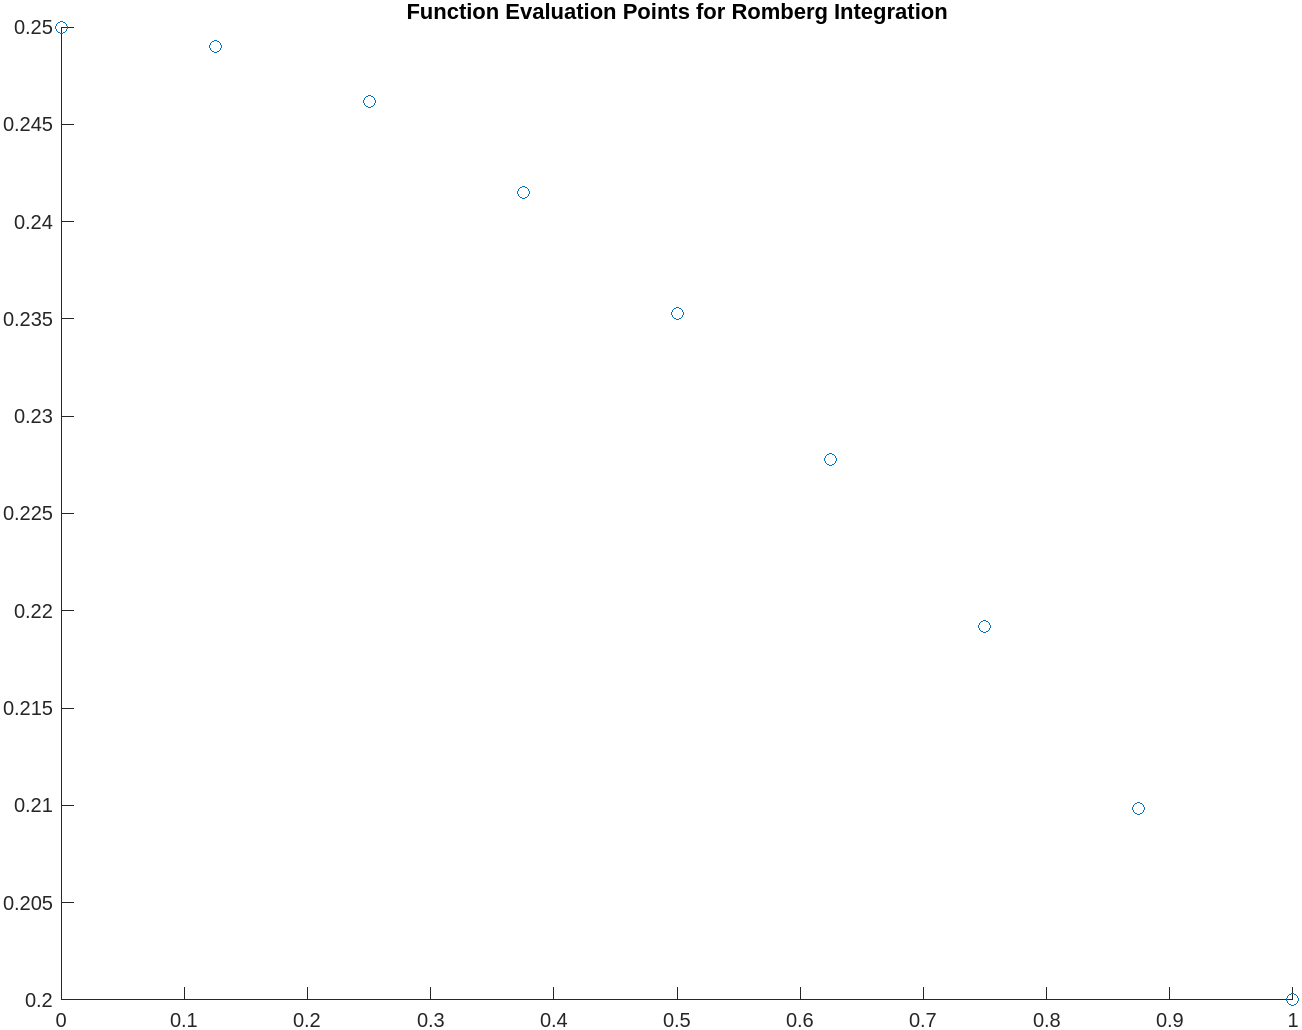
\includegraphics[width=0.8\textwidth]{q2}
    \caption{Points evaluated for final integral for question 2.}
    \label{fig:q2}
\end{figure}

{\medskip\noindent\bf Question 3.} Subtracting the first term of the Taylor series is already done for us in the question, so we just need to subtract the three term. $\cos x=1-\frac{x^2}{2}+\ldots$, so we want to evaluate
\[
I=\int_0^{\pi/2}x^{-\frac{1}{2}}dx-\int_0^{\pi/2}\frac{1}{2}x^{\frac{3}{2}}dx+\int_0^{\pi /2}\frac{1}{24}x^{7 /2}dx+\int_0^{\pi/2}x^{-\frac{1}{2}}\left( \cos x-1+\frac{x^2}{2}-\frac{x^{4}}{24}\right) dx
\]
\[
    =(2\pi)^{\frac{1}{2}}-\frac{\pi^{5 /2}}{20\sqrt{2}}+\frac{\pi^{9 /2}}{1728\sqrt{2}}+\int_0^{\pi/2}x^{-\frac{1}{2}}\left( \cos x-1+\frac{x^2}{2}-\frac{x^{4}}{24} \right) dx
.\]

Plugging in each of the methods previously coded for question 1, we get table \ref{tab:q3}. This is the code used to generate the table:
\begin{lstlisting}
f1 = @(x)x^(-0.5)*cos(x);
f2 = @(x)f2_func(x);
f3 = @(x)f3_func(x);

c1 = (2*pi)^0.5;
c2 = (2*pi)^0.5-pi^(5/2)/20/2^0.5+pi^(9/2)/1728/2^0.5;

N1 = 2^(4);
N2 = 2^(6);
a = 0;
b = pi/2;

T = zeros(8,2);

T(1,1) = midpoint_rule(f1,a,b,N1)
T(1,2) = midpoint_rule(f1,a,b,N2)

T(2,1) = gauss_legendre(f1,a,b,N1)
T(2,2) = gauss_legendre(f1,a,b,N2)

T(3,1) = midpoint_rule(f2,a,b,N1)+c1
T(3,2) = midpoint_rule(f2,a,b,N2)+c1

T(4,1) = gauss_legendre(f2,a,b,N1)+c1
T(4,2) = gauss_legendre(f2,a,b,N2)+c1

T(5,1) = trapezium_rule(f2,a,b,N1)+c1
T(5,2) = trapezium_rule(f2,a,b,N2)+c1

T(6,1) = midpoint_rule(f3,a,b,N1)+c2
T(6,2) = midpoint_rule(f3,a,b,N2)+c2

T(7,1) = gauss_legendre(f3,a,b,N1)+c2
T(7,2) = gauss_legendre(f3,a,b,N2)+c2

T(8,1) = trapezium_rule(f3,a,b,N1)+c2
T(8,2) = trapezium_rule(f3,a,b,N2)+c2

function ret = f2_func(x)
    if x == 0
        ret = 0;
    else
        ret = x^(-0.5)*(cos(x)-1);
    end
end

function ret = f3_func(x)
    if x == 0
        ret =  0;
    else
        ret = x^(-0.5)*(cos(x)-1+x^2/2-x^4/24);
    end
end

function result = midpoint_rule(f, a, b, N)
    result = 0;
    for i = 0:(N-1)
        point = a+(i+0.5)*(b-a)/N;
        result = result + f(point);
    end

    result = result * (b-a)/N;
end


function result = trapezium_rule(f, a, b, N)
    result = 0;
    for i = 1:(N-1)
        point = a+i*(b-a)/N;
        result = result + 2*f(point);
    end
    result = result + f(a) + f(b);

    result = result * (b-a)/N/2;
end

function result = simpsons_rule(f, a, b, N)
    result = 0;
    for i = 1:N
        left = a+(i-1)*(b-a)/N;
        right = a+i*(b-a)/N;
        result = result + 1/3*(b-a)/N/2*(f(left)+4*f((left+right)/2)+f(right));
    end
end

function result = gauss_legendre(f, a, b, N)
    x = [-sqrt(3/5), 0, sqrt(3/5)];
    w = [5/9, 8/9, 5/9];

    result = 0;
    for i = 1:N
        left = a + (i-1)*(b-a) / N;
        right = a + i*(b-a)/N;
        for j = 1:3
            xi = 0.5*(left+right + (right-left) * x(j));
            result = result+w(j)*f(xi);
        end
    end
    result = 0.5 * (b-a)/N*result;
end
\end{lstlisting}

\begin{table}
\centering
\begin{tabular}{|l|c|c|}
\hline
Integration Rule & \( h = \left(\frac{\pi}{2}\right)2^{-4} \) & \( h = \left(\frac{\pi}{2}\right)2^{-6} \) \\
\hline
Direct Midpoint & 1.765666396389619 & 1.860156095195565 \\
\hline
Direct 3 pt Gauss & 1.876839228294837 & 1.915870905333172 \\
\hline
Subtract 1 term Midpoint & 1.955096450291370 & 1.954915723360832 \\
\hline
Subtract 1 term 3 pt Gauss & 1.954903132541657 & 1.954902857457128 \\
\hline
Subtract 1 term Trapezium & 1.954504413769041 & 1.954876746967585 \\
\hline
Subtract 3 terms Midpoint & 1.954924860994853 & 1.954904226503539 \\
\hline
Subtract 3 terms 3 pt Gauss & 1.954902848582768 & 1.954902848582659 \\
\hline
Subtract 3 terms Trapezium & 1.954858792378667 & 1.954900092618298 \\
\hline
\end{tabular}
\caption{Question 3.}
\label{tab:q3}
\end{table}

{\medskip\noindent\bf Question 4.} See table \ref{tab:q4} for the filled in table and $\ref{fig:q4}$ for the plot. For the error of the discarded part, note that
\[
\left|\int_{c}^{\infty}f(r)J_0(kr)r dr\right|\leq \left|\int_{c}^{\infty}e^{-r}r dr\right|=(c+1)e^{-c}
.\]
Thus to obtain 4 digits of precision, assuming that the numerical integration of the first part is perfect (it can be arbitrarily good by increasing the number of iterations of Romberg integration), then we have that $(c+1)e^{-c}=10^{-4}\implies c=\log(c+1)+4\log 10$. This can be solved numerically using fixed point or Newton's method, which gives an answer of approximately $c=11.7$. Of course this is specific to the case of $f(r)=e^{-r}$, for a general function you'd have to put a bound on the integral $\int_c^{\infty}f(r)rdr$ The code used for this question is:

\begin{figure}[htpb]
    \centering
    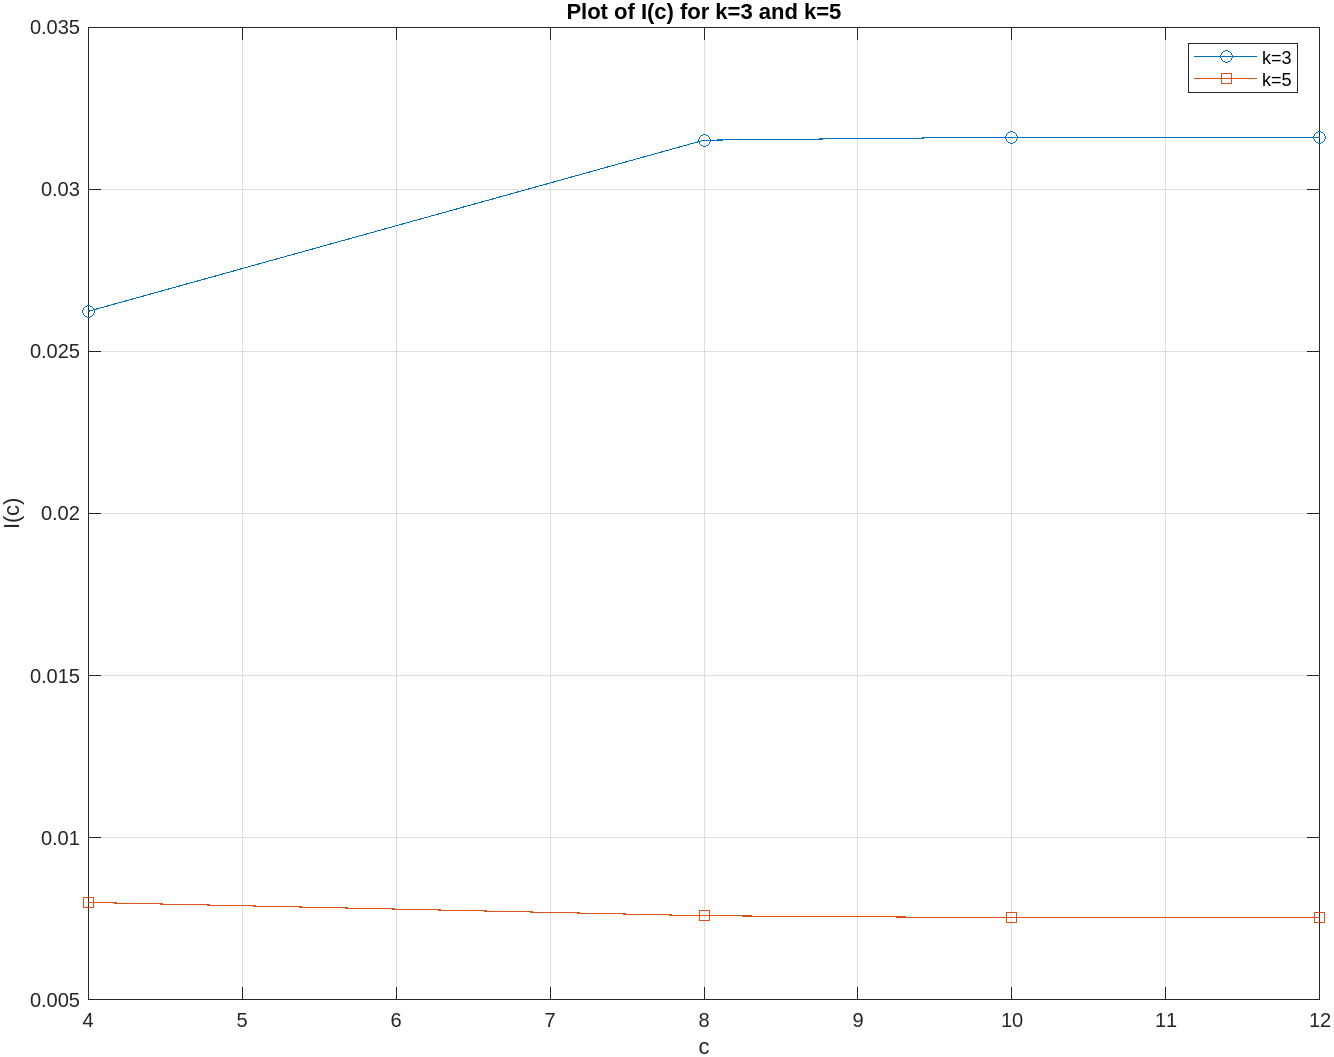
\includegraphics[width=0.8\textwidth]{q4}
    \caption{Plot for Question 4}
    \label{fig:q4}
\end{figure}

\begin{table}
\centering
\begin{tabular}{|l|c|c|}
\hline
\( k \) & 3 & 5 \\
\hline
\( c = 4 \) & 0.026232986735937 & 0.008007246646745 \\
\hline
\( c = 8 \) & 0.031513149602178 & 0.007596520009570 \\
\hline
\( c = 10 \) & 0.031607470669074 & 0.007534416688645 \\
\hline
\( c = 12 \) & 0.031593617989870 & 0.007545484466509 \\
\hline
Exact & 0.031622776601684 & 0.007542928274546 \\
\hline
\end{tabular}
\caption{Values for table of question 4.}
\label{tab:q4}
\end{table}

\begin{lstlisting}
f3 = @(r) exp(-r)*besselj(0,3*r)*r;
f5 = @(r) exp(-r)*besselj(0,5*r)*r;

c = [4, 8, 10, 12];
T3 = zeros(1, length(c));
T5 = zeros(1, length(c));

for i = 1:length(c)
    T3(i) = Romberg(f3, 0, c(i), 1e-4, 20);
    T5(i) = Romberg(f5, 0, c(i), 1e-4, 20);
end

plot(c, T3, 'o-', 'DisplayName', 'k=3');
hold on;
plot(c, T5, 's-', 'DisplayName', 'k=5');
hold off;

xlabel('c');
ylabel('I(c)');
title('Plot of I(c) for k=3 and k=5');
legend('Location', 'best');
grid on;

function Integral = Romberg(f,a,b,tol,kmax)
  I = zeros(kmax, kmax+1);
  for s=1:kmax
    I(s,1) = (b-a)/2^(s-1);
    % I(s,2) = trapez(f,a,b,2^(s-1));
  end

  k = 1;
  I(1,2) = trapez(f,a,b,1);
  I_last = I(2,1)+2*tol;
  I_cur = I(2,1);
  while abs(I_cur - I_last) >= tol && k<kmax
    k = k+1;
    I(k,2) = trapez(f,a,b,2^(k-1));
    for m=1:k-1
      I(k-m,m+2) = I(k-m+1,m+1) + (I(k-m+1,m+1)-I(k-m,m+1))/(4^m-1);
    end
    I_last = I_cur;
    I_cur = I(1,k+1);
  end

  Integral = I_last;
  X = a:(b-a)/2^(k-1):b;
end


function result = trapez(f, a, b, N)
    result = 0;
    for i = 1:(N-1)
        point = a+i*(b-a)/N;
        result = result + 2*f(point);
    end
    result = result + f(a) + f(b);

    result = result * (b-a)/N/2;
end
\end{lstlisting}

\end{document}
